% Given the dismal state of inter-paper comparisons, can we learn \textit{anything} from the existing work on neural network pruning? Our meta-analysis reveals that the answer is yes. % In this section, we discuss general lessons, findings surrounding the recently introduced \textit{lottery ticket hypothesis}, and novel findings mined from our aggregated results.

After aggregating results from a corpus of \npapers papers, we identified a number of consistent findings. In this section, we provide an overview of our corpus and then discuss these findings.

% ------------------------------------------------
\vspace{-.75mm}
\subsection{Papers Used in Our Analysis}
\vspace{-.25mm}
% ------------------------------------------------

Our corpus consists of 79 pruning papers published since 2010 and two classic papers \cite{optimal-brain-damage, optimal-brain-surgeon} that have been compared to by a number of recent methods. We selected these papers by identifying popular papers in the literature and what cites them, systematically searching through conference proceedings, and tracing the directed graph of comparisons between pruning papers. This last procedure results in the property that, barring oversights on our part, there is no pruning paper in our corpus that compares to any pruning paper outside of our corpus. Additional details about our corpus and its construction can be found in Appendix~\ref{sec:corpus}.

% We selected the \npapers papers used in our analysis in the following way. First, we conducted an ad hoc literature search, finding widely cited papers introducing pruning methods and identifying other pruning papers that cited them using Google Scholar. We then went through the conference proceedings from the past year's NeurIPS, ICML, CVPR, ECCV, and ICLR and added all papers we identified as being about pruning. Finally, during the course of cataloging which papers compared to which others, we added to our corpus any pruning paper that at least one existing paper in our corpus purported to compare to. We included both published papers and unpublished ones of reasonable quality (typically on arXiv).
% In short, we included essentially every reasonable-quality paper introducing a method of pruning neural networks that we could find, taking care to capture the full directed graph of papers and comparisons between them.

% ------------------------------------------------
\vspace{-1mm}
\subsection{How Effective is Pruning?}
\vspace{-.25mm}
% ------------------------------------------------

One of the clearest findings about pruning is that it works. More precisely, there are various methods that can significantly compress models with little or no loss of accuracy. In fact, for small amounts of compression, pruning can sometimes \textit{increase} accuracy \cite{learning-both, spectral-pruning}. This basic finding has been replicated in a large fraction of the papers in our corpus. % Plus, it has been found in conditions that control for most lurking variables we have discussed, since authors can compare the same model using the same code before and after pruning.
% is present in even in the first generation of pruning papers \cite{early-brain-damage, optimal-brain-surgeon},

Along the same lines, it has been repeatedly shown that, at least for large amounts of pruning, many pruning methods outperform random pruning \cite{nisp, google-state-of-sparsity, lottery-ticket-followup, divnet, apple-pfa, channel-lasso-lstsq}. Interestingly, this does not always hold for small amounts of pruning \cite{lottery-transfer}. Similarly, pruning all layers uniformly tends to perform worse than intelligently allocating parameters to different layers \cite{google-state-of-sparsity, learning-both, pruning-filters, nvidia-taylor-pruning, thinet-channel-norms} or pruning globally \cite{snip, lottery-ticket}. Lastly, when holding the number of fine-tuning iterations constant, many methods produce pruned models that outperform retraining from scratch with the same sparsity pattern \cite{zhang-accel-very-deep, nisp, bayesian-compression, channel-lasso-lstsq, thinet-channel-norms, lottery-ticket} (at least with a large enough amount of pruning \cite{apple-pfa}). Retraining from scratch in this context means training a fresh, randomly-initialized model with all weights clamped to zero throughout training, except those that are nonzero in the pruned model.

Another consistent finding is that sparse models tend to outperform dense ones for a fixed number of parameters. \citet{snip-followup} show that increasing the nominal size of ResNet-20 on CIFAR-10 while sparsifying to hold the number of parameters constant decreases the error rate. \citet{wavernn} obtain a similar result for audio synthesis, as do \citet{openai-block-sparse} for a variety of additional tasks across various domains. Perhaps most compelling of all are the many results, including in Figure~\ref{fig:arch_vs_prune}, showing that pruned models can obtain higher accuracies than the original models from which they are derived. This demonstrates that sparse models can not only outperform dense counterparts with the same number of parameters, but sometimes dense models with even more parameters.

% ------------------------------------------------
\subsection{Pruning vs Architecture Changes}
% ------------------------------------------------

One current unknown about pruning is how effective it tends to be relative to simply using a more efficient architecture. These options are not mutually exclusive, but it may be useful in guiding one's research or development efforts to know which choice is likely to have the larger impact. Along similar lines, it is unclear how pruned models from different architectures compare to one another---i.e., to what extent does pruning offer similar benefits across architectures?
% \begin{figure}[t]
% \begin{center}
% 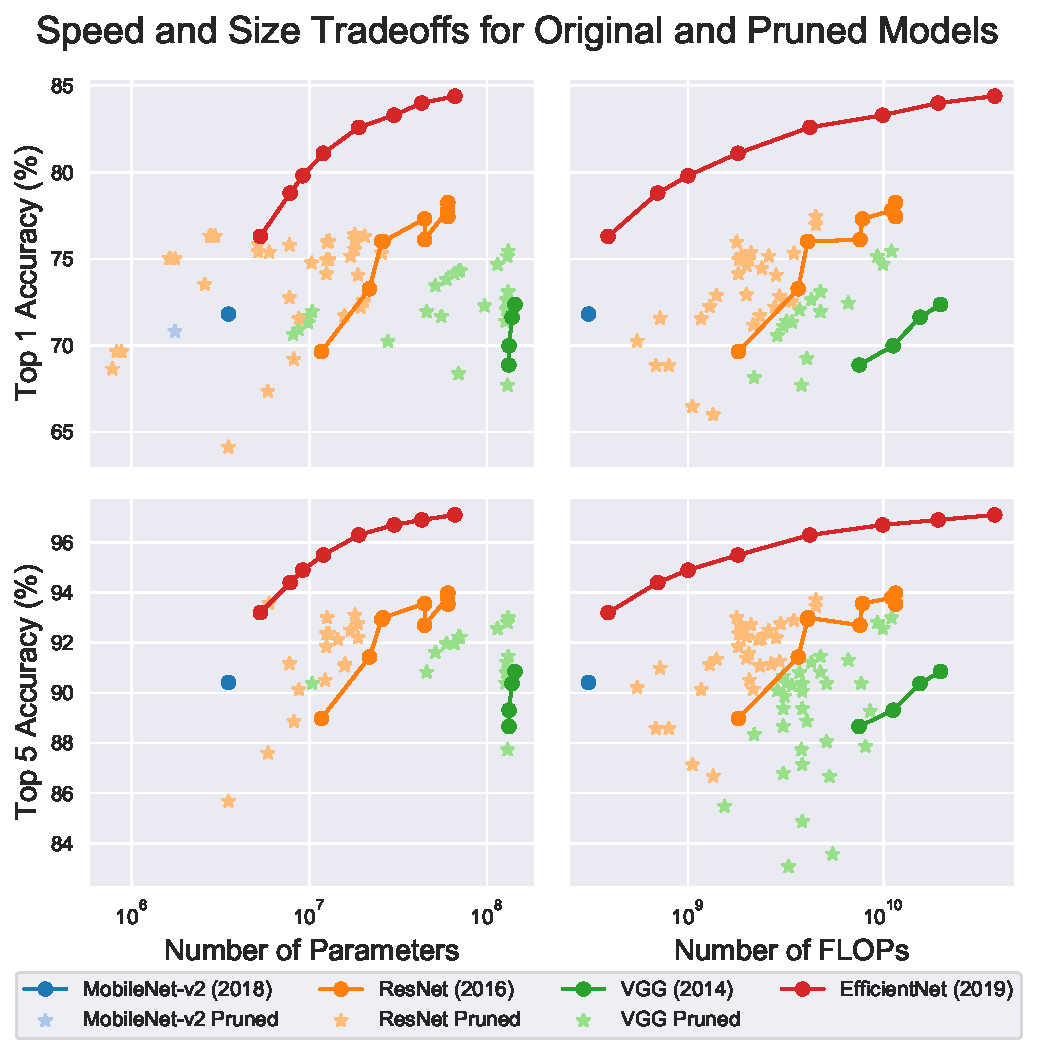
\includegraphics[width=\linewidth]{arch_vs_prune}
% \vspace{-3mm}
% \caption{Size and speed vs accuracy tradeoffs for different pruning methods and families of architectures. Pruned models sometimes outperform the original architecture, but rarely outperform a better architecture.}
% \label{fig:arch_vs_prune}
% \end{center}
% \end{figure}
To address these questions, we plotted the reported accuracies and compression/speedup levels of pruned models on ImageNet alongside the same metrics for different architectures with no pruning (Figure~\ref{fig:arch_vs_prune}).\footnote{
    Since many pruning papers report only change in accuracy or amount of pruning, without giving baseline numbers, we normalize all pruning results to have accuracies and model sizes/FLOPs as if they had begun with the same model. Concretely, this means multiplying the reported fraction of pruned size/FLOPs by a standardized initial value. This value is set to the median initial size or number of FLOPs reported for that architecture across all papers. This normalization scheme is not perfect, but does help control for different methods beginning with different baseline accuracies.
}
We plot results within a family of models as a single curve.\footnote{
    The EfficientNet family is given explicitly in the original paper \cite{efficientnet}, the ResNet family consists of ResNet-18, ResNet-34, ResNet-50, etc., and the VGG family consists of VGG-\{11, 13, 16, 19\}. There are no pruned EfficientNets since EfficientNet was published too recently. Results for non-pruned models are taken from \cite{efficientnet} and \cite{luigi}.
}

% We plot results within a family of models as a single curve. The EfficientNet family is given explicitly in the original paper \cite{efficientnet}, the ResNet family consists of ResNet-18, ResNet-34, ResNet-50, etc., and the VGG family consists of VGG-\{11, 13, 16, 19\}. There are no pruned EfficientNets since EfficientNet was published too recently. Results for non-pruned models are taken from \cite{efficientnet} and \cite{luigi}.

Figure~\ref{fig:arch_vs_prune} suggests several conclusions. First, it reinforces the conclusion that pruning can improve the time or space vs accuracy tradeoff of a given architecture, sometimes even increasing the accuracy. Second, it suggests that pruning generally does not help as much as switching to a better architecture. Finally, it suggests that pruning is more effective for architectures that are less efficient to begin with. % Finally, it suggests that pruning is more effective at reducing the size of models (left column) than their number of FLOPs (right column). This is unsurprising,

% \begin{figure}[t]
% \begin{center}
% 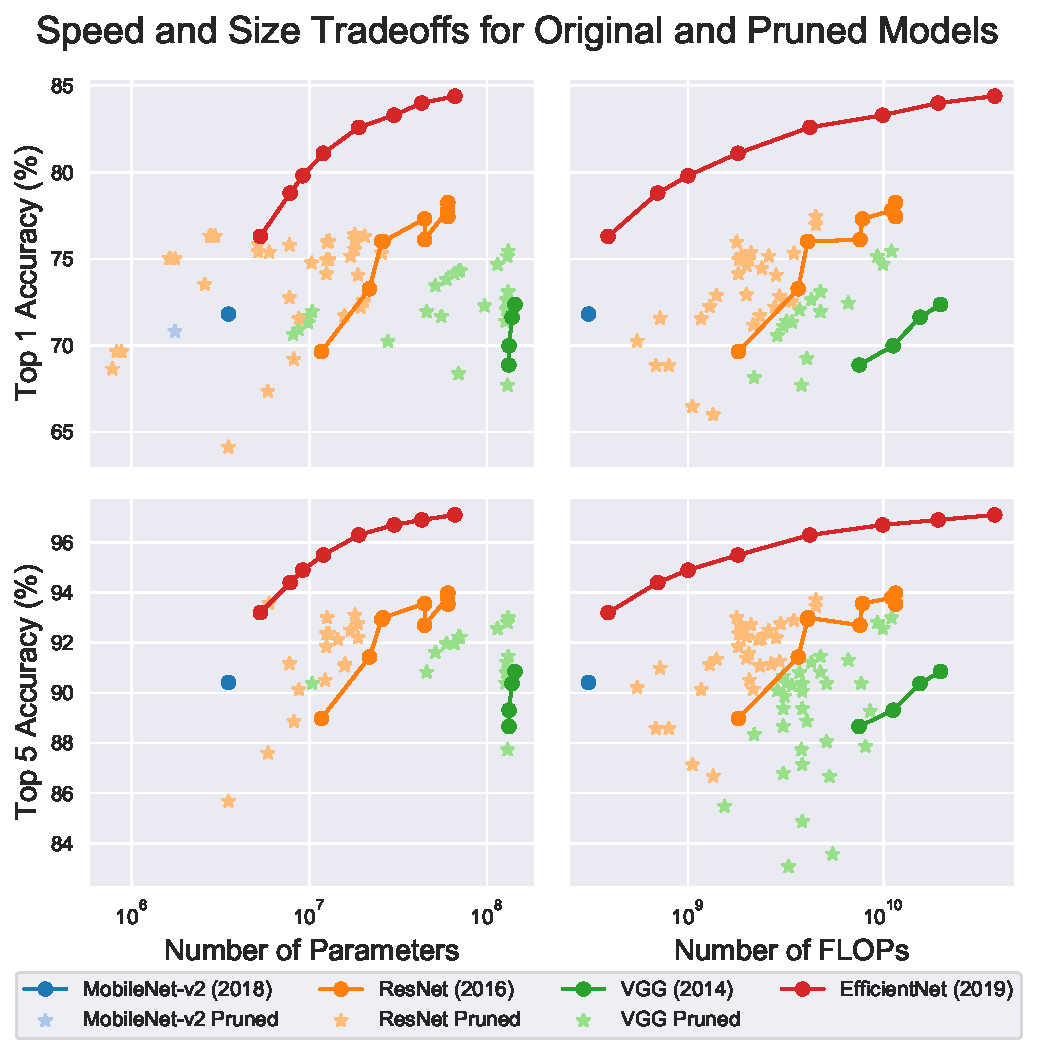
\includegraphics[width=\linewidth]{arch_vs_prune}
% \vspace{-3mm}
% \caption{Size and speed vs accuracy tradeoffs for different pruning methods and families of architectures. Pruned models sometimes outperform the original architecture, but rarely outperform a better architecture.}
% \label{fig:arch_vs_prune}
% \end{center}
% \end{figure}

% % ------------------------------------------------
% \subsection{Lottery Ticket Hypothesis}
% % ------------------------------------------------

% There has been a recent explosion of interest in the \textit{Lottery Ticket Hypothesis} \cite{lottery-ticket}. Informally, this hypothesis states that there are sparse subnetworks within a given model that 1) can be trained to equal or exceed the performance of the original model, and 2) depend on the initialization of the model, rather than merely the set of nonzeros chosen.
% The intuition behind the name is that these subnetworks have ``won the lottery'' with respect to initialization. Claim (1) follows from the general efficacy of pruning methods. Consequently, the investigation of the lottery ticket hypothesis centers on whether claim (2) holds; this is typically formulated as the question of whether retraining from scratch outperforms retraining from the pruned network's initial parameter values.
% % i.e., whether one must take into account the initialization when identifying the subnetwork, or whether it is only the pattern of nonzeros that matters.
% % As discussed above, the presence of a sparse subnetwork that outperforms the dense network has been demonstrated by numerous pruning papers.
% This question is interesting for at least two reasons:
% \begin{enumerate}
%     \itemsep2pt
%     \vspace{-3mm}
%     \item If the initialization from a fully-trained model significantly outperforms a random initialization, then obtaining peak efficiency requires a time consuming process of training and pruning. In contrast, if random initializations are just as good, one might be able to design or learn patterns of sparsity before running any training at all. \citet{snip} have already demonstrated that this is possible to some extent, though it does not yet appear to achieve the same performance as methods that use trained models \cite{lottery-ticket-followup}.
%     % \item If it is only the pattern of nonzeros that matters, it would likely be easier to design or learn patterns of nonzeros \textit{a priori} and obtain efficient, sparse models before running any training at all. [snip] has already demonstrated that this is possible to some extent, though it does not yet appear to achieve the same performance as methods that use the initialization or final trained model [lottery-ticket-followup].
%     \item The lottery ticket hypothesis is a bet against non-convex optimizers, in the sense that it holds only if the quality of the final solution depends on the initial parameter values. % To see this, consider that retraining from scratch should never perform worse that retraining from the initial parameter values given a sufficiently good optimizer, since the optimizer could, at the very least, begin
%     %1) if the lottery ticket hypothesis holds, a pruned network reset to its ``true'' initialization will outperform the same network reinitialized randomly; and 2) an oracle optimizer would obtain an equally good network regardless of the initialization. Therefore, we should expect the lottery ticket hypothesis to hold only if the optimizer used finds solutions of different quality depending on the initialization.
%     \vspace{-6mm}
% \end{enumerate}
% Multiple papers have confirmed the lottery ticket hypothesis for ResNet-50 on ImageNet \cite{google-state-of-sparsity, rethinking-net-pruning, stabilizing-lottery-tix}, and there is evidence that it holds for Transformer networks on language tasks \cite{google-state-of-sparsity} and other image classification networks on ImageNet \cite{lottery-transfer, lottery-ticket-followup}. However, the lottery ticket hypothesis does not always appear to hold. \citet{rethinking-net-pruning} show that retraining a pruned model from scratch can outperform the pruned model, and consistently does so  when allowing pruned models to train for longer than the original (so that the total number of \texttt{parameters} $\times$ \texttt{updates} remains close to constant). In light of this, recent work by Frankle \cite{lottery-ticket-followup, stabilizing-lottery-tix} (reproduced by \citet{lottery-transfer}) has shown that a simple modification of the lottery ticket hypothesis does always seem to hold. Namely, if instead of retraining from the initial parameter values, one retrains from the parameter values early in training (e.g., after one epoch), one consistently obtains a final model that outperforms those obtained by retraining from scratch. \citet{lottery-ticket-followup} also demonstrate that selecting which parameters to keep later in training tends to work better than doing so earlier.%, though selecting them only a few epochs into training can still yield a good pruned model.

% An interesting extension of the lottery ticket hypothesis is that of \cite{lottery-transfer}, who demonstrate that the sparse subnetworks in question can generalize across datasets and optimizers. In more detail, they show that if one prunes a neural network trained on one dataset, resets the non-pruned network parameters to their values early in training, and then trains this initial model on a new dataset (or with a new optimizer), the result is consistently better than randomly initializing the same network on the new dataset. Unsurprisingly, they find that initial models derived from larger datasets tend to yield better final accuracies than those from smaller datasets. More surprisingly, they find that initial models from \textit{large} datasets generalize better than initial models from the \textit{same} dataset when the latter dataset is small.

% % ------------------------------------------------
% \subsection{Other Findings}
% % ------------------------------------------------

% One consistent finding is that sparse models tend to outperform dense ones for a given number of parameters. \citet{snip-followup} show that increasing the nominal size of ResNet-20 on CIFAR-10 while sparsifying to hold the number of parameters constant decreases the error rate. \citet{wavernn} obtain a similar result for audio synthesis, as do \citet{openai-block-sparse} for a variety of additional tasks across various domains. Perhaps most compelling of all are the many results, including in Figure~\ref{fig:arch_vs_prune}, showing that pruned models can obtain higher accuracies than the original models from which they are derived. This demonstrates that sparse models can not only outperform dense counterparts with the same number of parameters, but sometimes dense models with even more parameters. % assuming one could add parameters to these models without harming their accuracies, these pruned models would also be instances of sparse models outperforming dense ones with the same number of parameters.

% There are also various credible findings in papers specifically attempting to improve the community's understanding of pruning in general.
% \citet{han-sparse-how} demonstrate that, for various models on large-scale image classification tasks, more granular sparsity consistently yields better accuracy for a given fraction of nonzeros. However, when measuring size by actual memory consumption instead of number of nonzeros, coarser sparsity can be better. This is because the latter reduces the overhead from storing nonzero indices by sharing one index between multiple nonzeros and sometimes reducing the necessary bit depth for indices.

% A more perplexing finding is that of \cite{prune-largest}. At least on CIFAR-10, they find that pruning the \textit{largest}-magnitude weights performs better than pruning the \textit{smallest}-magnitude weights, as long as the network is large enough to avoid underfitting. They show that this relates to the amount of ``instability'' introduced into the network, as measured by drop in validation accuracy immediately after pruning. This finding is surprising since pruning papers often frame their goal in terms of preserving the model's initial behavior. It is not yet clear how to reconcile this finding with the somewhat contrary result that current methods consistently perform better than random pruning (which one would expect to cause more instability).
